% Qwen3-8B forgetting and shape-regularization replications.
% Input by neurips_2025.tex in the appendix.

\section{Qwen3-8B Forgetting and Shape-Regularization Replications}
\label{app:qwen_forgetting}

This appendix reports the Qwen3-8B replications of Sec.~\ref{subsec:forget_exp} and Sec.~\ref{subsec:shape_reg_exp} along with the remaining trace-norm decomposition tables (Llama BBQ and both Qwen fine-tuning tasks). Qwen3-8B differs from Llama-3.1-8B in depth (36 vs.\ 32 layers), vocabulary size ($151{,}936$ vs.\ $128{,}256$), tokenizer family (byte-level BPE vs.\ BPE), and pre-training corpus (multilingual, $\sim$36T tokens vs.\ English-dominant, $\sim$15T tokens); reproducing the main-text patterns under these shifts provides cross-lineage evidence for the claims of Secs.~\ref{subsec:forget_exp}--\ref{subsec:shape_reg_exp}.

\subsection{Forgetting: Bound Tracks Cross-Task Drift on Qwen3-8B}
\label{app:qwen_forget_grid}

\begin{figure}[h]
    \centering
    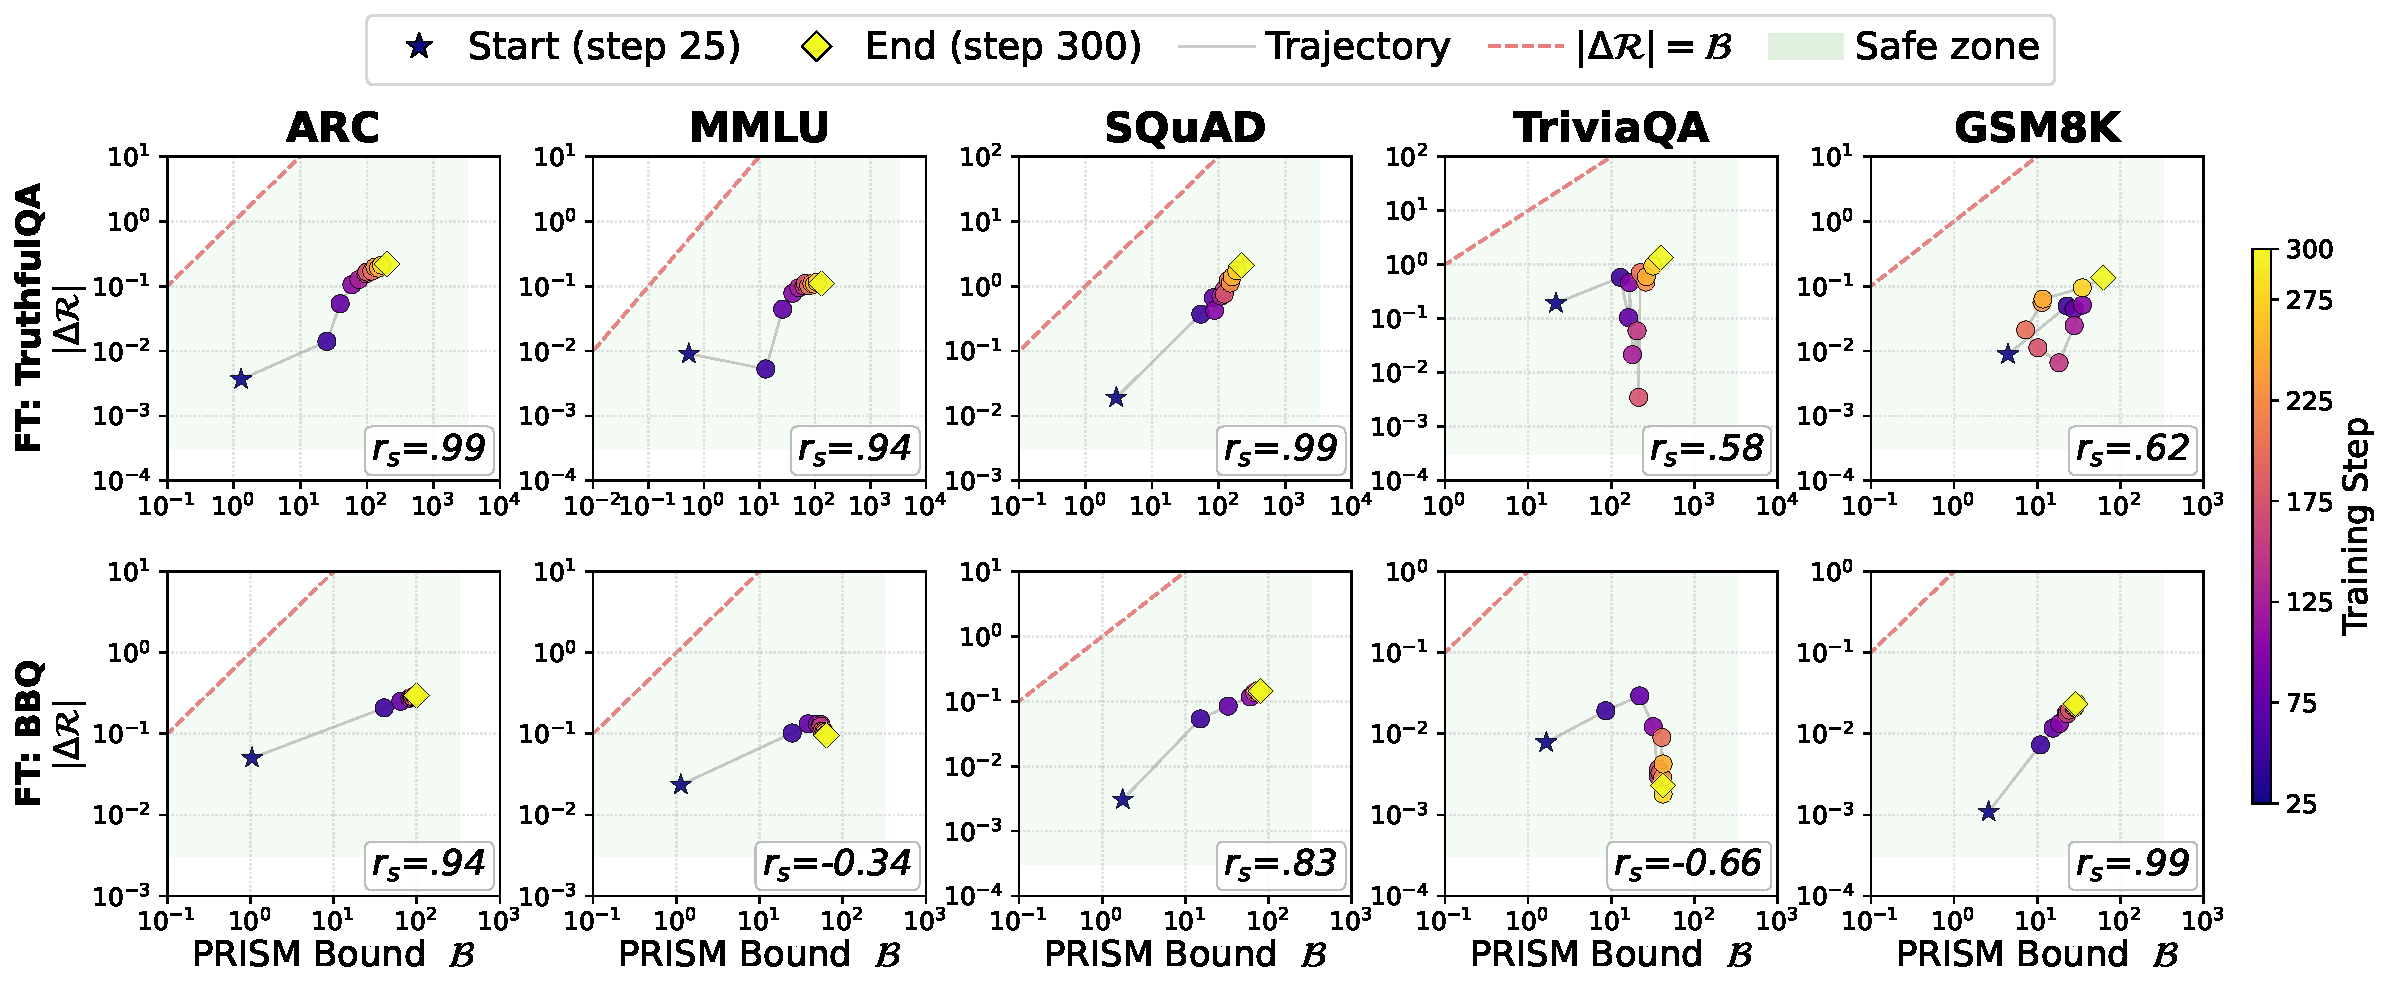
\includegraphics[width=1.0\linewidth]{figures/forgetting/forgetting_grid_bound_qwen.pdf}
    \caption{\textbf{Qwen3-8B: the PRISM bound tracks catastrophic forgetting across LoRA fine-tuning steps.} Each subplot scatters the PRISM bound $\mathcal{B}$ (x-axis, log) against the empirical forgetting $|\Delta\mathcal{R}|$ (y-axis, log) on a held-out benchmark, with one point per LoRA checkpoint colored by training step. Rows: fine-tuning task (TruthfulQA, BBQ). Columns: held-out evaluation benchmark (ARC, MMLU, SQuAD, TriviaQA, GSM8K). Because LoRA keeps the \texttt{lm\_head} frozen, the head-discrepancy term $\gamma$ vanishes and the bound is governed entirely by backbone scale ($\Delta\rho$) and shape ($1-\Omega$) drift, as predicted by Sec.~\ref{subsec:forgetting}. Spearman $r_s$ per subplot is annotated in each panel. This replicates Fig.~\ref{fig:forget_grid_llama} on a different lineage, whose pre-training corpus, depth, vocabulary size, and tokenizer family all differ from Llama-3.1-8B.}
    \label{fig:forget_grid_qwen}
\end{figure}

Figure~\ref{fig:forget_grid_qwen} reproduces the two structural observations of the Llama main-text result (Fig.~\ref{fig:forget_grid_llama}) on Qwen3-8B. First, \emph{the PRISM bound rises in lockstep with empirical forgetting across all $2\times 5$ (task, benchmark) combinations}: as LoRA fine-tuning proceeds on TruthfulQA or BBQ, $\Omega(Z_0, Z_t)$ drifts away from $1$ and $\rho_t$ from $\rho_0$, and this backbone drift tracks the empirical cross-entropy drift on every held-out benchmark---including benchmarks (e.g., GSM8K) whose distributions differ substantially from the fine-tuning data. Second, \emph{different source tasks induce qualitatively different drift geometries}, matching Llama: TruthfulQA fine-tuning drives predominantly shape drift while BBQ moves both scale and shape, a distinction the decomposition of Eq.~(\ref{eq:lora_bound}) makes visible whereas a unified distance would collapse it. Because Qwen3-8B differs from Llama-3.1-8B in every one of the four variables held out in Sec.~\ref{subsec:exp_setup} (pre-training corpus, depth, vocabulary, tokenizer family), this replication is direct evidence that the backbone-drift signal is a cross-family property rather than a Llama-specific artifact.

\subsection{Shape Regularization: Qwen3-8B Replication}
\label{app:qwen_shape_reg}

\begin{figure}[h]
    \centering
    
\includegraphics[width=1.0\linewidth]{figures/forgetting/combined_qwen_truthfulqa_bbq.pdf}
    \caption{\textbf{PRISM-guided shape regularization on Qwen3-8B (replication of Fig.~\ref{fig:shape_reg_combined_llama}).} LoRA fine-tuning on TruthfulQA (top row) and BBQ (bottom row) with the auxiliary penalty $\lambda(1-\Omega(Z_0^{\mathrm{ref}}, Z_t^{\mathrm{ref}}))$ at $\lambda \in \{0.0, 0.1, 0.5\}$ and analysis step $300$. The uniform downstream-forgetting reduction and the monotone trade-off between target-task fit and downstream damage seen on Llama hold on Qwen3-8B as well, confirming that the shape regularizer of Sec.~\ref{subsec:shape_reg} is not lineage-specific.}
    \label{fig:shape_reg_combined_qwen}
\end{figure}

\subsection{Additional Trace-Norm Decomposition Tables}
\label{app:trace_norm_tables}

Tables~\ref{tab:trace_norm_llama_bbq}--\ref{tab:trace_norm_qwen_bbq} give the full per-$(\text{model}, \text{fine-tuning task})$ decomposition at step $300$ for $\lambda \in \{0.0, 0.1, 0.5\}$. The main text (Table~\ref{tab:trace_norm_llama_truthfulqa}) showed the Llama-TruthfulQA combination; this appendix completes the $2\times 2$ grid.

\begin{table}[t]
\centering
\caption{Trace-norm forgetting decomposition for \textbf{Llama-3.1-8B} fine-tuned on \textbf{BBQ} under identity alignment ($W{=}I$).  Rows group by evaluation benchmark; each benchmark lists metrics at step 300 for $\lambda \in \{0.0, 0.1, 0.5\}$ (target $=$ base model).  Each benchmark also reports Spearman $r_s(\mathcal{B},\,|\Delta\mathcal{R}|)$ pooled across $\lambda \times$ checkpoints.}
\label{tab:trace_norm_llama_bbq}
\resizebox{\textwidth}{!}{%
\begin{tabular}{l l rrrrrrr}
\toprule
Dataset & $\lambda$ & $\rho_T$ & $\rho_P$ & $\Omega$ & $\delta$ & $\gamma$ & $\mathcal{B}$ & $|\Delta\mathcal{R}|$ \\
\midrule
BBQ (self) & $\lambda{=}0.0$ & 140.4590 & 142.6773 & \cellcolor{red!35} 0.6248 & \cellcolor{red!35} 122.6441 & \cellcolor{cyan!12} $0$ & \cellcolor{red!35} 122.6441 & \cellcolor{red!35} 1.0227 \\
{\small ($\mathbf{r_s{=}-0.18}$)} & $\lambda{=}0.1$ & 140.4590 & 141.5383 & \cellcolor{red!18} 0.8627 & \cellcolor{red!18} 73.8819 & \cellcolor{cyan!12} $0$ & \cellcolor{red!18} 193.1082 & \cellcolor{red!18} 1.0256 \\
 & $\lambda{=}0.5$ & 140.4590 & 141.0065 & \cellcolor{red!18} 0.9254 & \cellcolor{red!18} 54.3677 & \cellcolor{cyan!12} $0$ & \cellcolor{red!18} 142.1033 & \cellcolor{red!18} 1.0547 \\
\midrule
ARC & $\lambda{=}0.0$ & 137.5516 & 135.3145 & \cellcolor{red!18} 0.8762 & \cellcolor{red!18} 67.9234 & \cellcolor{cyan!12} $0$ & \cellcolor{red!18} 67.9234 & \cellcolor{red!18} 0.1884 \\
{\small ($\mathbf{r_s{=}-0.07}$)} & $\lambda{=}0.1$ & 137.5516 & 135.7115 & 0.9570 & 40.1190 & \cellcolor{cyan!12} $0$ & 104.8606 & 0.1846 \\
 & $\lambda{=}0.5$ & 137.5516 & 136.7454 & 0.9732 & 31.7369 & \cellcolor{cyan!12} $0$ & 82.9521 & 0.1892 \\
\midrule
MMLU & $\lambda{=}0.0$ & 138.9086 & 136.4845 & \cellcolor{red!18} 0.8759 & \cellcolor{red!18} 68.6286 & \cellcolor{cyan!12} $0$ & \cellcolor{red!18} 68.6286 & \cellcolor{red!18} 0.5218 \\
{\small ($\mathbf{r_s{=}0.10}$)} & $\lambda{=}0.1$ & 138.9086 & 137.1973 & 0.9563 & 40.8522 & \cellcolor{cyan!12} $0$ & 106.7771 & 0.6239 \\
 & $\lambda{=}0.5$ & 138.9086 & 138.2811 & 0.9724 & 32.5811 & \cellcolor{cyan!12} $0$ & 85.1586 & 0.5441 \\
\midrule
SQuAD & $\lambda{=}0.0$ & 138.1988 & 138.8436 & \cellcolor{red!18} 0.9429 & \cellcolor{red!18} 46.8184 & \cellcolor{cyan!12} $0$ & \cellcolor{red!18} 46.8184 & \cellcolor{red!18} 0.2117 \\
{\small ($\mathbf{r_s{=}0.80}$)} & $\lambda{=}0.1$ & 138.1988 & 138.8200 & 0.9508 & 43.4465 & \cellcolor{cyan!12} $0$ & 113.5579 & 0.4110 \\
 & $\lambda{=}0.5$ & 138.1988 & 138.5270 & 0.9633 & 37.4890 & \cellcolor{cyan!12} $0$ & 97.9867 & 0.3216 \\
\midrule
TriviaQA & $\lambda{=}0.0$ & 140.9310 & 141.5103 & 0.9841 & 25.2080 & \cellcolor{cyan!12} $0$ & 25.2080 & 0.1083 \\
{\small ($\mathbf{r_s{=}-0.03}$)} & $\lambda{=}0.1$ & 140.9310 & 141.3757 & 0.9892 & 20.7730 & \cellcolor{cyan!12} $0$ & 54.2951 & 0.0539 \\
 & $\lambda{=}0.5$ & 140.9310 & 141.1300 & 0.9945 & 14.7452 & \cellcolor{cyan!12} $0$ & 38.5401 & 0.0161 \\
\midrule
GSM8K & $\lambda{=}0.0$ & 137.1458 & 137.3618 & 1.0000 & 0.2161 & \cellcolor{cyan!12} $0$ & 0.2161 & 0.0478 \\
{\small ($\mathbf{r_s{=}-0.09}$)} & $\lambda{=}0.1$ & 137.1458 & 137.4127 & 1.0000 & 0.2669 & \cellcolor{cyan!12} $0$ & 0.6977 & 0.0300 \\
 & $\lambda{=}0.5$ & 137.1458 & 137.2236 & 1.0000 & 0.0778 & \cellcolor{cyan!12} $0$ & 0.2034 & 0.0152 \\
\bottomrule
\end{tabular}}
\end{table}

\begin{table}[t]
\centering
\caption{Trace-norm forgetting decomposition for \textbf{Qwen3-8B-Base} fine-tuned on \textbf{TruthfulQA} under identity alignment ($W{=}I$).  Rows group by evaluation benchmark; each benchmark lists metrics at step 300 for $\lambda \in \{0.0, 0.1, 0.5\}$ (target $=$ base model).  Each benchmark also reports Spearman $r_s(\mathcal{B},\,|\Delta\mathcal{R}|)$ pooled across $\lambda \times$ checkpoints.}
\label{tab:trace_norm_qwen_truthfulqa}
\resizebox{\textwidth}{!}{%
\begin{tabular}{l l rrrrrrr}
\toprule
Dataset & $\lambda$ & $\rho_T$ & $\rho_P$ & $\Omega$ & $\delta$ & $\gamma$ & $\mathcal{B}$ & $|\Delta\mathcal{R}|$ \\
\midrule
TruthfulQA (self) & $\lambda{=}0.0$ & 308.2324 & 248.8668 & \cellcolor{red!18} 0.8910 & \cellcolor{red!18} 142.2728 & \cellcolor{cyan!12} $0$ & \cellcolor{red!18} 142.2728 & \cellcolor{red!18} 0.3253 \\
{\small ($\mathbf{r_s{=}0.60}$)} & $\lambda{=}0.1$ & 308.2324 & 300.7398 & 0.9831 & 56.4401 & \cellcolor{cyan!12} $0$ & 195.1854 & 0.5458 \\
 & $\lambda{=}0.5$ & 308.2324 & 300.9807 & 0.9834 & 56.0154 & \cellcolor{cyan!12} $0$ & 193.7168 & 0.5473 \\
\midrule
ARC & $\lambda{=}0.0$ & 332.9777 & 316.0776 & 0.9854 & 58.0426 & \cellcolor{cyan!12} $0$ & 58.0426 & 0.2211 \\
{\small ($\mathbf{r_s{=}0.60}$)} & $\lambda{=}0.1$ & 332.9777 & 326.9742 & 0.9958 & 30.8029 & \cellcolor{cyan!12} $0$ & 106.5250 & 0.1727 \\
 & $\lambda{=}0.5$ & 332.9777 & 327.3377 & 0.9958 & 30.8393 & \cellcolor{cyan!12} $0$ & 106.6508 & 0.1678 \\
\midrule
MMLU & $\lambda{=}0.0$ & 333.5282 & 323.6556 & 0.9938 & 37.9230 & \cellcolor{cyan!12} $0$ & 37.9230 & 0.1110 \\
{\small ($\mathbf{r_s{=}0.76}$)} & $\lambda{=}0.1$ & 333.5282 & 328.7315 & 0.9983 & 19.9632 & \cellcolor{cyan!12} $0$ & 69.0384 & 0.1117 \\
 & $\lambda{=}0.5$ & 333.5282 & 328.9475 & 0.9983 & 19.8459 & \cellcolor{cyan!12} $0$ & 68.6326 & 0.1103 \\
\midrule
SQuAD & $\lambda{=}0.0$ & 297.6789 & 277.6624 & 0.9777 & 63.9596 & \cellcolor{cyan!12} $0$ & 63.9596 & 2.0940 \\
{\small ($\mathbf{r_s{=}0.48}$)} & $\lambda{=}0.1$ & 297.6789 & 292.4949 & 0.9927 & 36.0801 & \cellcolor{cyan!12} $0$ & 124.7748 & 0.9542 \\
 & $\lambda{=}0.5$ & 297.6789 & 292.8424 & 0.9930 & 35.3768 & \cellcolor{cyan!12} $0$ & 122.3427 & 0.9197 \\
\midrule
TriviaQA & $\lambda{=}0.0$ & 240.4206 & 201.6764 & \cellcolor{red!18} 0.8815 & \cellcolor{red!18} 113.9728 & \cellcolor{cyan!12} $0$ & \cellcolor{red!18} 113.9728 & \cellcolor{red!18} 1.3422 \\
{\small ($\mathbf{r_s{=}-0.26}$)} & $\lambda{=}0.1$ & 240.4206 & 224.4744 & 0.9655 & 63.0973 & \cellcolor{cyan!12} $0$ & 218.2079 & 0.1921 \\
 & $\lambda{=}0.5$ & 240.4206 & 224.9881 & 0.9661 & 62.4935 & \cellcolor{cyan!12} $0$ & 216.1197 & 0.1794 \\
\midrule
GSM8K & $\lambda{=}0.0$ & 269.0630 & 251.0654 & 1.0000 & 17.9976 & \cellcolor{cyan!12} $0$ & 17.9976 & 0.1352 \\
{\small ($\mathbf{r_s{=}0.20}$)} & $\lambda{=}0.1$ & 269.0630 & 272.5854 & 1.0000 & 3.5224 & \cellcolor{cyan!12} $0$ & 12.1813 & 0.0047 \\
 & $\lambda{=}0.5$ & 269.0630 & 272.3306 & 1.0000 & 3.2676 & \cellcolor{cyan!12} $0$ & 11.3001 & 0.0055 \\
\bottomrule
\end{tabular}}
\end{table}

\begin{table}[t]
\centering
\caption{Trace-norm forgetting decomposition for \textbf{Qwen3-8B-Base} fine-tuned on \textbf{BBQ} under identity alignment ($W{=}I$).  Rows group by evaluation benchmark; each benchmark lists metrics at step 300 for $\lambda \in \{0.0, 0.1, 0.5\}$ (target $=$ base model).  Each benchmark also reports Spearman $r_s(\mathcal{B},\,|\Delta\mathcal{R}|)$ pooled across $\lambda \times$ checkpoints.}
\label{tab:trace_norm_qwen_bbq}
\resizebox{\textwidth}{!}{%
\begin{tabular}{l l rrrrrrr}
\toprule
Dataset & $\lambda$ & $\rho_T$ & $\rho_P$ & $\Omega$ & $\delta$ & $\gamma$ & $\mathcal{B}$ & $|\Delta\mathcal{R}|$ \\
\midrule
BBQ (self) & $\lambda{=}0.0$ & 320.4945 & 282.7178 & 0.9742 & 78.0912 & \cellcolor{cyan!12} $0$ & 78.0912 & 0.2425 \\
{\small ($\mathbf{r_s{=}-0.36}$)} & $\lambda{=}0.1$ & 320.4945 & 287.7239 & 0.9863 & 60.0456 & \cellcolor{cyan!12} $0$ & 207.6543 & 0.2145 \\
 & $\lambda{=}0.5$ & 320.4945 & 294.7726 & 0.9915 & 47.6449 & \cellcolor{cyan!12} $0$ & 164.7692 & 0.2133 \\
\midrule
ARC & $\lambda{=}0.0$ & 332.9777 & 323.6521 & 0.9966 & 28.6389 & \cellcolor{cyan!12} $0$ & 28.6389 & 0.2959 \\
{\small ($\mathbf{r_s{=}0.72}$)} & $\lambda{=}0.1$ & 332.9777 & 325.0714 & 0.9977 & 23.6218 & \cellcolor{cyan!12} $0$ & 81.6908 & 0.2983 \\
 & $\lambda{=}0.5$ & 332.9777 & 325.8899 & 0.9983 & 20.4425 & \cellcolor{cyan!12} $0$ & 70.6960 & 0.2999 \\
\midrule
MMLU & $\lambda{=}0.0$ & 333.5282 & 327.6653 & 0.9986 & 18.4691 & \cellcolor{cyan!12} $0$ & 18.4691 & 0.0959 \\
{\small ($\mathbf{r_s{=}-0.38}$)} & $\lambda{=}0.1$ & 333.5282 & 328.6313 & 0.9990 & 15.5053 & \cellcolor{cyan!12} $0$ & 53.6217 & 0.0879 \\
 & $\lambda{=}0.5$ & 333.5282 & 329.2083 & 0.9990 & 15.3953 & \cellcolor{cyan!12} $0$ & 53.2413 & 0.0822 \\
\midrule
SQuAD & $\lambda{=}0.0$ & 297.6789 & 285.2593 & 0.9978 & 23.0185 & \cellcolor{cyan!12} $0$ & 23.0185 & 0.1444 \\
{\small ($\mathbf{r_s{=}0.38}$)} & $\lambda{=}0.1$ & 297.6789 & 286.0710 & 0.9985 & 19.7367 & \cellcolor{cyan!12} $0$ & 68.2550 & 0.1337 \\
 & $\lambda{=}0.5$ & 297.6789 & 287.0676 & 0.9990 & 16.9506 & \cellcolor{cyan!12} $0$ & 58.6198 & 0.1312 \\
\midrule
TriviaQA & $\lambda{=}0.0$ & 240.4206 & 235.3667 & 0.9989 & 12.1057 & \cellcolor{cyan!12} $0$ & 12.1057 & 0.0023 \\
{\small ($\mathbf{r_s{=}-0.18}$)} & $\lambda{=}0.1$ & 240.4206 & 235.4420 & 0.9991 & 11.1248 & \cellcolor{cyan!12} $0$ & 38.4726 & 0.0013 \\
 & $\lambda{=}0.5$ & 240.4206 & 235.6737 & 0.9992 & 10.5391 & \cellcolor{cyan!12} $0$ & 36.4471 & 0.0055 \\
\midrule
GSM8K & $\lambda{=}0.0$ & 269.0630 & 260.6926 & 1.0000 & 8.3704 & \cellcolor{cyan!12} $0$ & 8.3704 & 0.0233 \\
{\small ($\mathbf{r_s{=}0.87}$)} & $\lambda{=}0.1$ & 269.0630 & 261.3101 & 1.0000 & 7.7529 & \cellcolor{cyan!12} $0$ & 26.8118 & 0.0254 \\
 & $\lambda{=}0.5$ & 269.0630 & 262.1636 & 1.0000 & 6.8995 & \cellcolor{cyan!12} $0$ & 23.8602 & 0.0242 \\
\bottomrule
\end{tabular}}
\end{table}
